% 7 Appendix C
\section{Appendix C}

\begin{guidance}
\centering
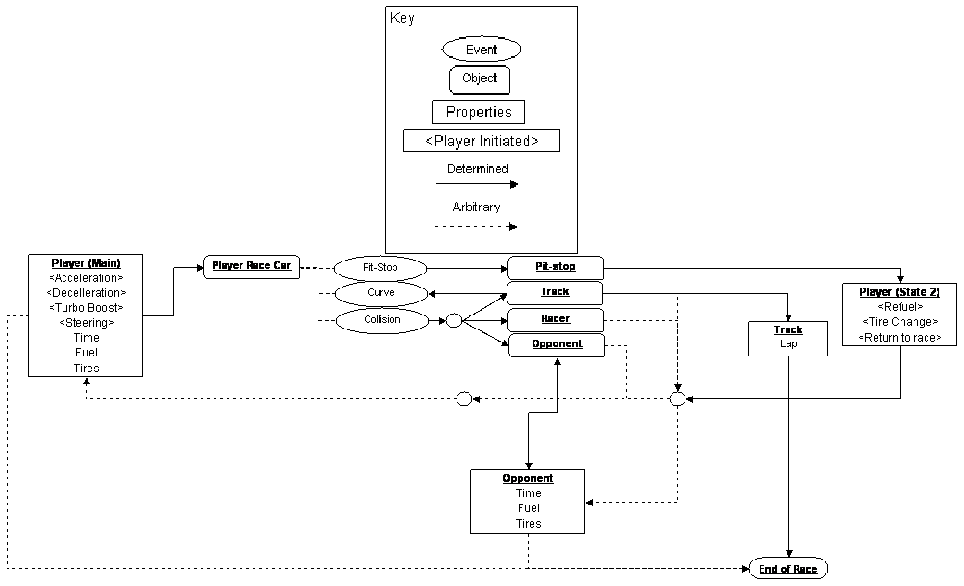
\includegraphics[width=\linewidth,height=0.82\textheight,keepaspectratio]{figures/appendix-c-flow-chart.pdf}
\end{guidance}
% Write your text below.

\subsection{Hold the Door -- Game Flow Chart}

The flow chart below illustrates the complete operational loop of \textbf{Hold the Door}, representing the states, decision nodes, and transitions between player actions, zombie lifecycle, tower interactions, and fence preservation.

\begin{figure}[htbp]
\centering
\begin{tikzpicture}[
  node distance=1.1cm and 1.3cm,
  terminal/.style={rectangle, rounded corners=6pt, draw=black!80, fill=gddhead, thick, text width=2.4cm, align=center, inner sep=5pt, font=\small\bfseries},
  process/.style={rectangle, draw=black!80, fill=white, thick, text width=2.5cm, align=center, inner sep=5pt, font=\small},
  decision/.style={diamond, aspect=1.8, draw=black!80, fill=gddlabel, thick, text width=2.0cm, align=center, inner sep=2pt, font=\footnotesize\bfseries},
  arrow/.style={-{Stealth[scale=1.0]}, thick, draw=black!80}
]

% Nodes
\node (start) [terminal] {Start Game / Select Level};
\node (prep) [process, below=of start] {\textbf{Preparation Phase}\\Inspect Sockets\\Build / Upgrade\\Towers (Scrap)};
\node (call) [decision, below=of prep] {Call Wave\\or Timer?};
\node (combat) [process, below=of call] {\textbf{Combat Phase}\\Spawn Zombies\\Move Left $\rightarrow$ Right};
\node (tower) [process, left=of combat] {\textbf{Towers Target}\\Single / Sniper / Shotgun; Fire bullets/pellets};
\node (hit) [decision, below=of combat] {Zombie\\Defeated?};
\node (bounty) [process, left=of hit] {\textbf{Collect Bounty}\\+Scrap to Treasury\\Play Death SFX};
\node (reach) [decision, below=of hit] {Reached\\The Fence?};
\node (dmg) [process, right=of reach] {\textbf{Fence Damaged}\\Subtract Fence HP\\Crash SFX / Shake};
\node (dead) [decision, below=of reach] {Fence HP\\$\le 0$?};
\node (defeat) [terminal, right=of dead, fill=red!20] {\textbf{DEFEAT}\\Fence Broken\\Retry / Exit};
\node (wavecheck) [decision, below=of dead] {Horde\\Cleared?};
\node (lastwave) [decision, below=of wavecheck] {Final\\Wave?};
\node (victory) [terminal, right=of lastwave, fill=green!20] {\textbf{VICTORY}\\Award 1--3 Stars\\Unlock Next Stage};

% Connections
\draw [arrow] (start) -- (prep);
\draw [arrow] (prep) -- (call);
\draw [arrow] (call) -- node[right, font=\footnotesize] {Yes} (combat);
\draw [arrow] (call.west) -- ++(-0.6,0) |- node[near end, left, font=\footnotesize] {Adjust} (prep.west);

\draw [arrow] (combat) -- (hit);
\draw [arrow] (combat.west) -- (tower.east);
\draw [arrow] (tower.south) |- (hit.west);

\draw [arrow] (hit) -- node[above, font=\footnotesize] {Yes} (bounty);
\draw [arrow] (bounty.north) |- (prep.west);
\draw [arrow] (hit) -- node[right, font=\footnotesize] {No} (reach);

\draw [arrow] (reach) -- node[above, font=\footnotesize] {Yes} (dmg);
\draw [arrow] (dmg) |- (dead);
\draw [arrow] (reach) -- node[left, font=\footnotesize] {No} (dead);

\draw [arrow] (dead) -- node[above, font=\footnotesize] {Yes} (defeat);
\draw [arrow] (dead) -- node[right, font=\footnotesize] {No} (wavecheck);

\draw [arrow] (wavecheck.west) -- ++(-1.8,0) |- node[near end, left, font=\footnotesize] {More zombies} (combat.west);
\draw [arrow] (wavecheck) -- node[right, font=\footnotesize] {Wave done} (lastwave);

\draw [arrow] (lastwave) -- node[above, font=\footnotesize] {Yes} (victory);
\draw [arrow] (lastwave.west) -- ++(-2.4,0) |- node[near end, left, font=\footnotesize] {Next wave prep} (prep.west);

\end{tikzpicture}
\caption{System Gameplay Flowchart of \textbf{Hold the Door}}
\label{fig:game-flowchart}
\end{figure}
